\documentclass{article}
\usepackage{tikz}

\usepackage{pgfplots,pgfplotstable}
%\usepackage[pdftex]{graphicx} 
% set up externalization
\usetikzlibrary{external}


\pgfplotstableread[col sep = comma]{CSV/Scalability_2obj.csv}\ScalabilityTwoObj
\pgfplotstableread[col sep = comma]{CSV/Scalability_3obj.csv}\ScalabilityThreeObj
\pgfplotstableread[col sep = comma]{CSV/Initial_Distance_Factor_HV.csv}\DIHV
\pgfplotstableread[col sep = comma]{CSV/Initial_Distance_Factor_IGDP.csv}\DIIGDP
\pgfplotstableread[col sep = comma]{CSV/Diversity2obj.csv}\DiversityTwoWFG
\pgfplotstableread[col sep = comma]{CSV/Diversity3obj.csv}\DiversityThreeWFG
%\pgfplotstableread[col sep = comma]{CSV/Diversity2objWFG5.csv}\DiversityTwoWFGFive
%\pgfplotstableread[col sep = comma]{CSV/Diversity3objWFG5.csv}\DiversityThreeWFGFive
%\pgfplotstableread[col sep = comma]{CSV/Diversity2objWFG6.csv}\DiversityTwoWFGSix
%\pgfplotstableread[col sep = comma]{CSV/Diversity3objWFG6.csv}\DiversityThreeWFGSix
\pgfplotstableread[col sep = comma]{CSV/PerformanceTime2obj.csv}\Performancetimetwo
\pgfplotstableread[col sep = comma]{CSV/PerformanceTime3obj.csv}\Performancetimethree



\tikzset{external/system call={latex \tikzexternalcheckshellescape -halt-on-error
-interaction=batchmode -jobname "\image" "\texsource";
dvips -o "\image".ps "\image".dvi;
ps2eps "\image.ps"}}
\tikzexternalize
\begin{document}
%



%\tikzset{every picture/.style={line width=0.75pt}} %set default line width to 0.75pt        

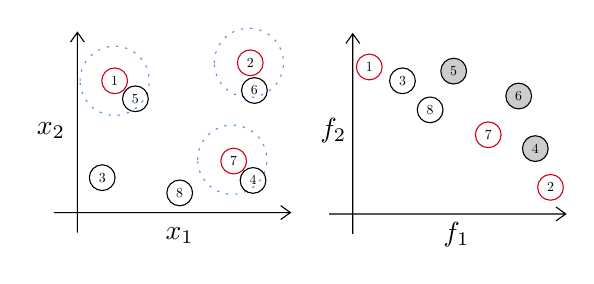
\begin{tikzpicture}[x=0.5pt,y=0.5pt,yscale=-1,xscale=1]
%uncomment if require: \path (0,300); %set diagram left start at 0, and has height of 300

%Shape: Circle [id:dp5136866411017809] 
\draw  [color={rgb, 255:red, 74; green, 144; blue, 226 }  ,draw opacity=1 ][dash pattern={on 0.84pt off 2.51pt}] (69,105) .. controls (69,91.19) and (80.19,80) .. (94,80) .. controls (107.81,80) and (119,91.19) .. (119,105) .. controls (119,118.81) and (107.81,130) .. (94,130) .. controls (80.19,130) and (69,118.81) .. (69,105) -- cycle ;
%Shape: Circle [id:dp3061612047883613] 
\draw  [color={rgb, 255:red, 74; green, 144; blue, 226 }  ,draw opacity=1 ][dash pattern={on 0.84pt off 2.51pt}] (166,92) .. controls (166,78.19) and (177.19,67) .. (191,67) .. controls (204.81,67) and (216,78.19) .. (216,92) .. controls (216,105.81) and (204.81,117) .. (191,117) .. controls (177.19,117) and (166,105.81) .. (166,92) -- cycle ;
%Shape: Axis 2D [id:dp3645341276574614] 
\draw  (50,200.22) -- (221,200.22)(67.1,70) -- (67.1,214.69) (214,195.22) -- (221,200.22) -- (214,205.22) (62.1,77) -- (67.1,70) -- (72.1,77)  ;
%Shape: Circle [id:dp595877391054507] 
\draw  [color={rgb, 255:red, 74; green, 144; blue, 226 }  ,draw opacity=1 ][dash pattern={on 0.84pt off 2.51pt}] (154,162) .. controls (154,148.19) and (165.19,137) .. (179,137) .. controls (192.81,137) and (204,148.19) .. (204,162) .. controls (204,175.81) and (192.81,187) .. (179,187) .. controls (165.19,187) and (154,175.81) .. (154,162) -- cycle ;
%Shape: Axis 2D [id:dp14963900792703488] 
\draw  (249,201.22) -- (420,201.22)(266.1,71) -- (266.1,215.69) (413,196.22) -- (420,201.22) -- (413,206.22) (261.1,78) -- (266.1,71) -- (271.1,78)  ;

% Text Node
\draw  [color={rgb, 255:red, 208; green, 2; blue, 27 }  ,draw opacity=1 ]  (94, 105) circle [x radius= 9.3, y radius= 9.3]   ;
\draw (94,105) node [scale=0.5] [align=left] {1};
% Text Node
\draw  [color={rgb, 255:red, 0; green, 0; blue, 0 }  ,draw opacity=1 ]  (109, 118) circle [x radius= 9.3, y radius= 9.3]   ;
\draw (109,118) node [scale=0.5] [align=left] {5};
% Text Node
\draw  [color={rgb, 255:red, 208; green, 2; blue, 27 }  ,draw opacity=1 ]  (192, 92) circle [x radius= 9.3, y radius= 9.3]   ;
\draw (192,92) node [scale=0.5] [align=left] {2};
% Text Node
\draw    (195, 112) circle [x radius= 9.3, y radius= 9.3]   ;
\draw (195,112) node [scale=0.5] [align=left] {6};
% Text Node
\draw  [color={rgb, 255:red, 208; green, 2; blue, 27 }  ,draw opacity=1 ]  (180, 163) circle [x radius= 9.3, y radius= 9.3]   ;
\draw (180,163) node [scale=0.5] [align=left] {7};
% Text Node
\draw    (194, 177) circle [x radius= 9.3, y radius= 9.3]   ;
\draw (194,177) node [scale=0.5] [align=left] {4};
% Text Node
\draw    (141, 186) circle [x radius= 9.3, y radius= 9.3]   ;
\draw (141,186) node [scale=0.5] [align=left] {8};
% Text Node
\draw    (85, 175) circle [x radius= 9.3, y radius= 9.3]   ;
\draw (85,175) node [scale=0.5] [align=left] {3};
% Text Node
\draw  [color={rgb, 255:red, 208; green, 2; blue, 27 }  ,draw opacity=1 ]  (278, 95) circle [x radius= 9.3, y radius= 9.3]   ;
\draw (278,95) node [scale=0.5] [align=left] {1};
% Text Node
\draw  [color={rgb, 255:red, 0; green, 0; blue, 0 }  ,draw opacity=1 ][fill={rgb, 255:red, 0; green, 0; blue, 0 }  ,fill opacity=0.2 ]  (339, 98) circle [x radius= 9.3, y radius= 9.3]   ;
\draw (339,98) node [scale=0.5] [align=left] {5};
% Text Node
\draw  [color={rgb, 255:red, 208; green, 2; blue, 27 }  ,draw opacity=1 ]  (409, 182) circle [x radius= 9.3, y radius= 9.3]   ;
\draw (409,182) node [scale=0.5] [align=left] {2};
% Text Node
\draw  [fill={rgb, 255:red, 0; green, 0; blue, 0 }  ,fill opacity=0.2 ]  (386, 116) circle [x radius= 9.3, y radius= 9.3]   ;
\draw (386,116) node [scale=0.5] [align=left] {6};
% Text Node
\draw  [color={rgb, 255:red, 208; green, 2; blue, 27 }  ,draw opacity=1 ]  (364, 144) circle [x radius= 9.3, y radius= 9.3]   ;
\draw (364,144) node [scale=0.5] [align=left] {7};
% Text Node
\draw  [fill={rgb, 255:red, 0; green, 0; blue, 0 }  ,fill opacity=0.2 ]  (398, 154) circle [x radius= 9.3, y radius= 9.3]   ;
\draw (398,154) node [scale=0.5] [align=left] {4};
% Text Node
\draw    (322, 126) circle [x radius= 9.3, y radius= 9.3]   ;
\draw (322,126) node [scale=0.5] [align=left] {8};
% Text Node
\draw    (302, 105) circle [x radius= 9.3, y radius= 9.3]   ;
\draw (302,105) node [scale=0.5] [align=left] {3};
% Text Node
\draw (141,217) node   {$x_{1}$};
% Text Node
\draw (48,141) node   {$x_{2}$};
% Text Node
\draw (341,216) node   {$f_{1}$};
% Text Node
\draw (252,141) node   {$f_{2}$};


\end{tikzpicture}



\begin{tikzpicture}[scale=0.8]
\begin{axis}[
ymin=0.5,
%ymax=1.1,
%x label style={at={(current axis.left of origin)},anchor=north, below=10mm},
title={\textit{\textbf{Scalability with Two Objectives}}},
    xlabel=Number of Decision Variables,
  ylabel=Mean HV,
%  xlabel style={yshift=-0.2cm},
  xticklabel style = {rotate=30},
  legend style=
    {cells={anchor=east},legend pos=outer north east,},
  % enlargelimits = false,
  xticklabels from table={\ScalabilityTwoObj}{mean},xtick=data]
  
\addplot[red,solid,mark=square*] 
table [y=VSD_MOEA_D,x=X]{\ScalabilityTwoObj};
\addlegendentry{AVSD-MOEA/D}
%\addplot[blue,dotted,mark=triangle*] table[y= NSGA_II,x=X]{\ScalabilityTwoObj};
%\addlegendentry{NSGA-II}]
%		
%\addplot[orange,dashed,mark=diamond*] table [y= R2_MOEA,x=X]{\ScalabilityTwoObj};
%\addlegendentry{R2-EMOA}]
    
\addplot[black,loosely dotted,mark=pentagon*] table [y= MOEA_D,x=X]{\ScalabilityTwoObj};
\addlegendentry{MOEA/D-DE}]
\end{axis}
\end{tikzpicture}
%\begin{tikzpicture}[scale=0.8]
%\begin{axis}[
%%ymin=0.5    ,
%%ymax=1.1,
%%x label style={at={(current axis.left of origin)},anchor=north, below=10mm},
%title={\textit{\textbf{Scalability UF5}}},
%    xlabel=Number of Decision Variables,
%  ylabel=Mean HV,
%  xticklabel style = {rotate=30},
%  legend style=
%    {cells={anchor=east},legend pos=outer north east,},
%  % enlargelimits = false,
%  xticklabels from table={\ScalabilityUFFiveTwoObj}{mean},xtick=data]
%  
%\addplot[red,solid,mark=square*] 
%table [y=VSD_MOEA,x=X]{\ScalabilityUFFiveTwoObj};
%\addlegendentry{VSD-MOEA}
%\addplot[blue,dotted,mark=triangle*] table [y= NSGA_II,x=X]{\ScalabilityUFFiveTwoObj};
%\addlegendentry{NSGA-II}]
%		
%\addplot[orange,dashed,mark=diamond*] table [y= R2_MOEA,x=X]{\ScalabilityUFFiveTwoObj};
%\addlegendentry{R2-MOEA}]
%    
%\addplot[black,loosely dotted,mark=pentagon*] table [y= MOEA_D,x=X]{\ScalabilityUFFiveTwoObj};
%\addlegendentry{MOEA/D}]
%\end{axis}
%\end{tikzpicture}
%\caption{Mean of the \HV{} (35 runs) considering two objectives.}


%\begin{figure}[t]
%\centering
%\begin{tikzpicture}[scale=0.8]
\begin{axis}[
ymin=0.0,
title={\textit{\textbf{Scalability with Three Objectives}}},
    xlabel=Number of Decision Variables,
  ylabel=Mean HV,
%  xlabel style={yshift=-0.2cm},
  xticklabel style = {rotate=30},
  legend style=
    {cells={anchor=east},legend pos=outer north east,},
  xticklabels from table={\ScalabilityThreeObj}{mean},xtick=data]
  
\addplot[red,solid,mark=square*] 
table [y=VSD_MOEA_D,x=X]{\ScalabilityThreeObj};
\addlegendentry{VSD-MOEA/D}
%\addplot[blue,dotted,mark=triangle*] table [y= NSGA_II,x=X]{\ScalabilityThreeObj};
%\addlegendentry{NSGA-II}]
%		
%\addplot[orange,dashed,mark=diamond*] table [y= R2_MOEA,x=X]{\ScalabilityThreeObj};
%\addlegendentry{R2-EMOA}]
    
\addplot[black,loosely dotted,mark=pentagon*] table [y= MOEA_D,x=X]{\ScalabilityThreeObj};
\addlegendentry{MOEA/D-DE}]
\end{axis}
\end{tikzpicture}
%\begin{tikzpicture}[scale=0.8]
%\begin{axis}[
%ymin=0.0,
%title={\textit{\textbf{Scalability UF10}}},
%    xlabel=Number of Decision Variables,
%  ylabel=Mean HV,
%  xticklabel style = {rotate=30},
%  legend style=
%    {cells={anchor=east},legend pos=outer north east,},
%  xticklabels from table={\ScalabilityUFTenThreeObj}{mean},xtick=data]
%  
%\addplot[red,solid,mark=square*] 
%table [y=VSD_MOEA,x=X]{\ScalabilityUFTenThreeObj};
%\addlegendentry{VSD-MOEA}
%\addplot[blue,dotted,mark=triangle*] table [y= NSGA_II,x=X]{\ScalabilityUFTenThreeObj};
%\addlegendentry{NSGA-II}]
%		
%\addplot[orange,dashed,mark=diamond*] table [y= R2_MOEA,x=X]{\ScalabilityUFTenThreeObj};
%\addlegendentry{R2-MOEA}]
%    
%\addplot[black,loosely dotted,mark=pentagon*] table [y= MOEA_D,x=X]{\ScalabilityUFTenThreeObj};
%\addlegendentry{MOEA/D}]
%\end{axis}
%\end{tikzpicture}
%\caption{Mean of the \HV{} (35 runs) considering three objectives.}

%\label{fig:variable-decision-scalability-3obj}
%\end{figure}
%
%
%\begin{figure}[t]
%\centering
%\begin{tikzpicture}[scale=0.8]
\begin{axis}[
title={\textit{\textbf{Diversity of the Position Variables with Two Objectives}}},
  xlabel=Function Evaluations,
  ylabel=ADI,
  xticklabel style = {rotate=30},
%  xlabel style={yshift=-0.2cm},
  legend style=
    {cells={anchor=east},legend pos=outer north east,}, nodes={scale=0.8, transform shape}    ,
  xticklabels from table={\DiversityTwoWFG}{mean},xtick=data]
 

\addplot[red,dotted,mark=square*] table [y=VSD_MOEA_Position_50,x=X]{\DiversityTwoWFG};
	\addlegendentry{VSD-MOEA (50)}

\addplot[blue,dotted,mark=triangle*] table[y= NSGA_II_Position_50,x=X]{\DiversityTwoWFG};
	\addlegendentry{NSGA-II (50)}
		
\addplot[orange,dotted,mark=diamond*] table [y= R2_MOEA_Position_50,x=X]{\DiversityTwoWFG};
	\addlegendentry{R2-EMOA (50)}
    
\addplot[black,dotted,mark=pentagon*] table [y= MOEA_D_Position_50,x=X]{\DiversityTwoWFG};
	\addlegendentry{MOEA/D (50)}


\addplot[red,solid,mark=square*] table [y=VSD_MOEA_Position_100,x=X]{\DiversityTwoWFG};
	\addlegendentry{VSD-MOEA (100)}

\addplot[blue,solid,mark=triangle*] table[y= NSGA_II_Position_100,x=X]{\DiversityTwoWFG};
	\addlegendentry{NSGA-II (100)}
		
\addplot[orange,solid,mark=diamond*] table [y= R2_MOEA_Position_100,x=X]{\DiversityTwoWFG};
	\addlegendentry{R2-EMOA (100)}
    
\addplot[black,solid,mark=pentagon*] table [y= MOEA_D_Position_100,x=X]{\DiversityTwoWFG};
	\addlegendentry{MOEA/D (100)}


\addplot[red,loosely dashdotted,mark=square*] table [y=VSD_MOEA_Position_250,x=X]{\DiversityTwoWFG};
	\addlegendentry{VSD-MOEA (250)}

\addplot[blue,loosely dashdotted,mark=triangle*] table[y= NSGA_II_Position_250,x=X]{\DiversityTwoWFG};
	\addlegendentry{NSGA-II (250)}
		
\addplot[orange,loosely dashdotted,mark=diamond*] table [y= R2_MOEA_Position_250,x=X]{\DiversityTwoWFG};
	\addlegendentry{R2-EMOA (250)}
    
\addplot[black,loosely dashdotted,mark=pentagon*] table [y= MOEA_D_Position_250,x=X]{\DiversityTwoWFG};
	\addlegendentry{MOEA/D (250)}



\end{axis}
\end{tikzpicture}


\begin{tikzpicture}[scale=0.8]
\begin{axis}[
title={\textit{\textbf{Diversity of the Distance Variables with Two Objectives}}},
  xlabel=Function Evaluations,
  ylabel=ADI,
%  xlabel style={yshift=-0.2cm},
  xticklabel style = {rotate=30},
  legend style=
    {cells={anchor=east},legend pos=outer north east,}, nodes={scale=0.8, transform shape}    ,
  xticklabels from table={\DiversityTwoWFG}{mean},xtick=data]

\addplot[red,dotted,mark=square*] table [y=VSD_MOEA_Distance_50,x=X]{\DiversityTwoWFG};
	\addlegendentry{VSD-MOEA (50)}

%\addplot[blue,dotted,mark=triangle*] table[y= NSGA_II_Distance_50,x=X]{\DiversityTwoWFG};
%	\addlegendentry{NSGA-II (50)}
		
\addplot[orange,dotted,mark=diamond*] table [y= R2_MOEA_Distance_50,x=X]{\DiversityTwoWFG};
	\addlegendentry{R2-EMOA (50)}
    
%\addplot[black,dotted,mark=pentagon*] table [y= MOEA_D_Distance_50,x=X]{\DiversityTwoWFG};
%	\addlegendentry{MOEA/D (50)}


\addplot[red,solid,mark=square*] table [y=VSD_MOEA_Distance_100,x=X]{\DiversityTwoWFG};
	\addlegendentry{VSD-MOEA (100)}

%\addplot[blue,solid,mark=triangle*] table[y= NSGA_II_Distance_100,x=X]{\DiversityTwoWFG};
%	\addlegendentry{NSGA-II (100)}
		
\addplot[orange,solid,mark=diamond*] table [y= R2_MOEA_Distance_100,x=X]{\DiversityTwoWFG};
	\addlegendentry{R2-EMOA (100)}
    
%\addplot[black,solid,mark=pentagon*] table [y= MOEA_D_Distance_100,x=X]{\DiversityTwoWFG};
%	\addlegendentry{MOEA/D (100)}


\addplot[red,loosely dashdotted,mark=square*] table [y=VSD_MOEA_Distance_250,x=X]{\DiversityTwoWFG};
	\addlegendentry{VSD-MOEA (250)}

%\addplot[blue,loosely dashdotted,mark=triangle*] table[y= NSGA_II_Distance_250,x=X]{\DiversityTwoWFG};
%	\addlegendentry{NSGA-II (250)}
		
\addplot[orange,loosely dashdotted,mark=diamond*] table [y= R2_MOEA_Distance_250,x=X]{\DiversityTwoWFG};
	\addlegendentry{R2-EMOA (250)}
    
%\addplot[black,loosely dashdotted,mark=pentagon*] table [y= MOEA_D_Distance_250,x=X]{\DiversityTwoWFG};
%	\addlegendentry{MOEA/D (250)}





\end{axis}
\end{tikzpicture}

%%\begin{tikzpicture}[scale=0.8]
%%\begin{axis}[
%%title={\textit{\textbf{Diversity of the Variables}}},
%%  xlabel=Generation,
%%  ylabel=ADI,
%%  xticklabel style = {rotate=30},
%%  legend style=
%%    {cells={anchor=east},legend pos=outer north east,},
%%  xticklabels from table={\DiversityTwoWFGOne}{mean},xtick=data]
%%
%%\addplot[red,dotted,mark=square*] table [y=VSD_MOEA,x=X]{\DiversityTwoWFGOne};
%%\addlegendentry{VSD-MOEA}
%%
%%\addplot[blue,dotted,mark=triangle*] table[y= NSGA_II,x=X]{\DiversityTwoWFGOne};
%%\addlegendentry{NSGA-II}
%%		
%%\addplot[orange,dotted,mark=diamond*] table [y= R2_MOEA,x=X]{\DiversityTwoWFGOne};
%%\addlegendentry{R2-MOEA}
%%    
%%\addplot[black,dotted,mark=pentagon*] table [y= MOEA_D,x=X]{\DiversityTwoWFGOne};
%%\addlegendentry{MOEA/D}
%%
%%
%%\addplot[red,solid,mark=square*] table [y=VSD_MOEA,x=X]{\DiversityThreeWFGOne};
%%\addlegendentry{VSD-MOEA}
%%
%%\addplot[blue,solid,mark=triangle*] table[y= NSGA_II,x=X]{\DiversityThreeWFGOne};
%%\addlegendentry{NSGA-II}
%%		
%%\addplot[orange,solid,mark=diamond*] table [y= R2_MOEA,x=X]{\DiversityThreeWFGOne};
%%\addlegendentry{R2-MOEA}
%%    
%%\addplot[black,solid,mark=pentagon*] table [y= MOEA_D,x=X]{\DiversityThreeWFGOne};
%%\addlegendentry{MOEA/D}
%%
%%	
%%\end{axis}
%%\end{tikzpicture}
%\caption{Evolution of Average Distance Individuals of the Problems WFG1-WFG7.}


%\label{fig:Diversity_2obj}
%\end{figure}
%
%
%\begin{figure}[t]
%\centering
%\begin{tikzpicture}[scale=0.8]
\begin{axis}[
title={\textit{\textbf{Diversity of the Position Variables with Three Objectives}}},
  xlabel=Function Evaluations,
  ylabel=ADI,
%  xlabel style={yshift=-0.2cm},
 xticklabel style = {rotate=30},
  legend style=
   {cells={anchor=east},legend pos=outer north east,}, nodes={scale=0.8, transform shape}    ,
    %{cells={anchor=east},legend pos=outer north east,},
  xticklabels from table={\DiversityThreeWFG}{mean},xtick=data]
 

\addplot[red,dotted,mark=square*] table [y=VSD_MOEA_Position_50,x=X]{\DiversityThreeWFG};
	\addlegendentry{VSD-MOEA (50)}

\addplot[blue,dotted,mark=triangle*] table[y= NSGA_II_Position_50,x=X]{\DiversityThreeWFG};
	\addlegendentry{NSGA-II (50)}
		
\addplot[orange,dotted,mark=diamond*] table [y= R2_MOEA_Position_50,x=X]{\DiversityThreeWFG};
	\addlegendentry{R2-EMOA (50)}
    
\addplot[black,dotted,mark=pentagon*] table [y= MOEA_D_Position_50,x=X]{\DiversityThreeWFG};
	\addlegendentry{MOEA/D (50)}


\addplot[red,solid,mark=square*] table [y=VSD_MOEA_Position_100,x=X]{\DiversityThreeWFG};
	\addlegendentry{VSD-MOEA (100)}

\addplot[blue,solid,mark=triangle*] table[y= NSGA_II_Position_100,x=X]{\DiversityThreeWFG};
	\addlegendentry{NSGA-II (100)}
		
\addplot[orange,solid,mark=diamond*] table [y= R2_MOEA_Position_100,x=X]{\DiversityThreeWFG};
	\addlegendentry{R2-EMOA (100)}
    
\addplot[black,solid,mark=pentagon*] table [y= MOEA_D_Position_100,x=X]{\DiversityThreeWFG};
	\addlegendentry{MOEA/D (100)}


\addplot[red,loosely dashdotted,mark=square*] table [y=VSD_MOEA_Position_250,x=X]{\DiversityThreeWFG};
	\addlegendentry{VSD-MOEA (250)}

\addplot[blue,loosely dashdotted,mark=triangle*] table[y= NSGA_II_Position_250,x=X]{\DiversityThreeWFG};
	\addlegendentry{NSGA-II (250)}
		
\addplot[orange,loosely dashdotted,mark=diamond*] table [y= R2_MOEA_Position_250,x=X]{\DiversityThreeWFG};
	\addlegendentry{R2-EMOA (250)}
    
\addplot[black,loosely dashdotted,mark=pentagon*] table [y= MOEA_D_Position_250,x=X]{\DiversityThreeWFG};
	\addlegendentry{MOEA/D (250)}



\end{axis}
\end{tikzpicture}


\begin{tikzpicture}[scale=0.8]
\begin{axis}[
title={\textit{\textbf{Diversity of the Distance Variables with Three Objectives}}},
  xlabel=Function Evaluations,
  ylabel=ADI,
  xticklabel style = {rotate=30},
%  xlabel style={yshift=-0.2cm},
  legend style=
   {cells={anchor=east},legend pos=outer north east,}, nodes={scale=0.8, transform shape}    ,
    %{cells={anchor=east},legend pos=outer north east,},
  xticklabels from table={\DiversityThreeWFG}{mean},xtick=data]

\addplot[red,dotted,mark=square*] table [y=VSD_MOEA_Distance_50,x=X]{\DiversityThreeWFG};
	\addlegendentry{VSD-MOEA (50)}

%\addplot[blue,dotted,mark=triangle*] table[y= NSGA_II_Distance_50,x=X]{\DiversityThreeWFG};
%	\addlegendentry{NSGA-II (50)}
		
\addplot[orange,dotted,mark=diamond*] table [y= R2_MOEA_Distance_50,x=X]{\DiversityThreeWFG};
	\addlegendentry{R2-EMOA (50)}
    
%\addplot[black,dotted,mark=pentagon*] table [y= MOEA_D_Distance_50,x=X]{\DiversityThreeWFG};
%	\addlegendentry{MOEA/D (50)}


\addplot[red,solid,mark=square*] table [y=VSD_MOEA_Distance_100,x=X]{\DiversityThreeWFG};
	\addlegendentry{VSD-MOEA (100)}

%\addplot[blue,solid,mark=triangle*] table[y= NSGA_II_Distance_100,x=X]{\DiversityThreeWFG};
%	\addlegendentry{NSGA-II (100)}
		
\addplot[orange,solid,mark=diamond*] table [y= R2_MOEA_Distance_100,x=X]{\DiversityThreeWFG};
	\addlegendentry{R2-EMOA (100)}
    
%\addplot[black,solid,mark=pentagon*] table [y= MOEA_D_Distance_100,x=X]{\DiversityThreeWFG};
%	\addlegendentry{MOEA/D (100)}


\addplot[red,loosely dashdotted,mark=square*] table [y=VSD_MOEA_Distance_250,x=X]{\DiversityThreeWFG};
	\addlegendentry{VSD-MOEA (250)}

%\addplot[blue,loosely dashdotted,mark=triangle*] table[y= NSGA_II_Distance_250,x=X]{\DiversityThreeWFG};
%	\addlegendentry{NSGA-II (250)}
		
\addplot[orange,loosely dashdotted,mark=diamond*] table [y= R2_MOEA_Distance_250,x=X]{\DiversityThreeWFG};
	\addlegendentry{R2-EMOA (250)}
    
%\addplot[black,loosely dashdotted,mark=pentagon*] table [y= MOEA_D_Distance_250,x=X]{\DiversityThreeWFG};
%	\addlegendentry{MOEA/D (250)}





\end{axis}
\end{tikzpicture}

%%\begin{tikzpicture}[scale=0.8]
%%\begin{axis}[
%%title={\textit{\textbf{Diversity of the Variables}}},
%%  xlabel=Generation,
%%  ylabel=ADI,
%%  xticklabel style = {rotate=30},
%%  legend style=
%%    {cells={anchor=east},legend pos=outer north east,},
%%  xticklabels from table={\DiversityThreeWFGOne}{mean},xtick=data]
%%
%%\addplot[red,dotted,mark=square*] table [y=VSD_MOEA,x=X]{\DiversityThreeWFGOne};
%%\addlegendentry{VSD-MOEA}
%%
%%\addplot[blue,dotted,mark=triangle*] table[y= NSGA_II,x=X]{\DiversityThreeWFGOne};
%%\addlegendentry{NSGA-II}
%%		
%%\addplot[orange,dotted,mark=diamond*] table [y= R2_MOEA,x=X]{\DiversityThreeWFGOne};
%%\addlegendentry{R2-MOEA}
%%    
%%\addplot[black,dotted,mark=pentagon*] table [y= MOEA_D,x=X]{\DiversityThreeWFGOne};
%%\addlegendentry{MOEA/D}
%%
%%
%%\addplot[red,solid,mark=square*] table [y=VSD_MOEA,x=X]{\DiversityThreeWFGOne};
%%\addlegendentry{VSD-MOEA}
%%
%%\addplot[blue,solid,mark=triangle*] table[y= NSGA_II,x=X]{\DiversityThreeWFGOne};
%%\addlegendentry{NSGA-II}
%%		
%%\addplot[orange,solid,mark=diamond*] table [y= R2_MOEA,x=X]{\DiversityThreeWFGOne};
%%\addlegendentry{R2-MOEA}
%%    
%%\addplot[black,solid,mark=pentagon*] table [y= MOEA_D,x=X]{\DiversityThreeWFGOne};
%%\addlegendentry{MOEA/D}
%%
%%	
%%\end{axis}
%%\end{tikzpicture}
%\caption{Evolution of Average Distance Individuals of the Problems WFG1-WFG7.}

%\label{fig:Diversity_3obj}
%\end{figure}
%
%
%\begin{figure}[t]
%\centering
%\input{Graphic-Performance-Time.tex}
%\label{fig:Performance_time}
%\end{figure}
%
%
%
%\begin{figure}[t]
%\centering
%\begin{tikzpicture}[scale=0.8]
\begin{axis}[
title={\textit{\textbf{Mean of the HV Value with Several Initial Threshold Values}}},
    xlabel=Initial Threshold Value,
  ylabel=Mean HV,
%  xlabel style={yshift=-0.2cm},
  xticklabel style = {rotate=30},
  legend style=
    {cells={anchor=east},legend pos=outer north east,},
  xticklabels from table={\DIHV}{mean},xtick=data]
  
\addplot[red,solid,mark=square*] 
table [y=HV2obj,x=X]{\DIHV};
\addlegendentry{HV - 2obj}
\addplot[blue,dotted,mark=triangle*] table[y= HV3obj,x=X]{\DIHV};
\addlegendentry{HV - 3obj}
		
\end{axis}
\end{tikzpicture}
%%\begin{tikzpicture}[scale=0.8]
%%\begin{axis}[
%%ymin=0.0    ,
%%ymax=0.1,
%%title={\textit{\textbf{Mean of the IGD+ Value with Several Initial Distance Factor}}},
%%    xlabel=Initial Distance Factor,
%%  ylabel=IGD+,
%%  xticklabel style = {rotate=30},
%%  legend style=
%%    {cells={anchor=east},legend pos=outer north east,},
%%  xticklabels from table={\DIIGDP}{mean},xtick=data]
%%\addplot[red,solid,mark=square*] 
%%table [y=IGD2obj,x=X]{\DIIGDP};
%%\addlegendentry{IGD+ 2obj}
%%\addplot[blue,dotted,mark=triangle*] table [y=IGD3obj,x=X]{\DIIGDP};
%%\addlegendentry{IGD+ 3obj}
%%\end{axis}
%%\end{tikzpicture}
%\caption{Mean of Inidicator Considering All Instances with Several Initial Distance Factors}

%\label{fig:Initial-distance-factor}
%\end{figure}

\end{document}
